\documentclass{article} 
\usepackage[left=0.75in,top=0.6in,right=0.75in,bottom=0.6in]{geometry} % Document margins
\usepackage{tabularx}
\usepackage{fancyvrb}
\usepackage{graphicx}
\usepackage{multicol,caption}
\usepackage{fancyhdr}
\usepackage{lipsum}
\usepackage{mathtools}

%Header Stuff
\newenvironment{Figure}
  {\par\medskip\noindent\ignorespaces\minipage{\linewidth}}
  {\endminipage\par\medskip}

\usepackage{fancyhdr}
\pagestyle{fancy}
\fancyhf{}
\renewcommand{\headrulewidth}{0pt}
\fancyhead[R]{\thepage}


\begin{document}

%----------------------------------------------------------------------------------------
%		 TITLE 
%----------------------------------------------------------------------------------------
\begin{center}

\vspace* {15 pt}
\Huge{\bf Image Processing: Overlaying and Histogram Equalization}\\
\vspace {20 pt}
\large{Howard Edwards, Michael Micros, Jonathon  Rigney, Megan Rowland \\}

\end{center}

\vspace{20 pt}




\begin{multicols*}{2}

%----------------------------------------------------------------------------------------
%		ABSTRACT
%----------------------------------------------------------------------------------------
{\bf  \textit {Abstract(Howard Edwards)} --- This report covers basic image processing. Two C++ command line programs were created that load 8-bit grayscale images for processing. Each program is able to process an image and produce a new image that is visibly different from the original. The programs create image files displaying the end result of the processed image. The image processing is done in two distinctive manner: image overlaying and histogram equalization. Image overlaying is done by adding an image, selected by the user, on top of the original input image. The user-selected image maybe words, such as subtitles, or pictures, such as a logo. Histogram equalization involves modifying an image intensities to improve contrast using the image’s histogram. An image’s histogram refers to the number of pixels for each intensity value of that image represented graphically.
}\\

{\bf  \textit {Index Terms} --- Gray-scale, Image analysis, Image processing
}



%----------------------------------------------------------------------------------------
%		INTRODUCTION
%----------------------------------------------------------------------------------------

\begin{center}
\large{I. Introduction(Jonathon Rigney)}
\end{center}

{The goal of the research being done is to design,  build, test and demonstrate an integrated system that performs real-time video processing based on field-programmable gating arrays (FPGAs) and is controlled via a graphical user interface (GUI) on a PC. Probably the most important aspect of real-time video processing is the manipulation of each frame that is received from the input stream. This paper deals with the implementation of two types of image (frame) processing which are: 1) Overlaying each frame of the video with a user-selected image, and 2) histogram equalization of each video frame. The goals that were set for this implementation were met with good results for both image overlay and histogram equalization.
}

%----------------------------------------------------------------------------------------
%		DESIGN
%----------------------------------------------------------------------------------------

\begin{center}
{\large II. Design (Megan Rowland)}
\end{center}

{\bf A. Summary of Design--}  
The overall design consists of an Image class to input and output a BMP file, a function to compute histogram equalization of an image and a function to overlay two images. The image class can be seen in Fig.9 of the Appendix 

{\bf B. Detail Description}\\
{\bf Inputting an Image:}
Executing the command line program will first prompt for the filename of an 8-bit BMP grayscale image file.. This image will be used for the original image. Next, there will be a prompt to enter the filename of an overlay image that is the same size as the original image. 
Example runs of the command line program for both test1.bmp and test2.bmp can be seen in Fig. 1 and Fig. 2.\\
First, from main(), the first 8-bit grayscale image file is read into, with the function readBM(), an instance of the Image class named original. The readBM function initializes the data types for that image. The data types include the width of the image (imageWidth), the height of the image (imageHeight), the amount of bits for the image (imageBits), the offset between the header and the pixels of the image (offset), a vector of all of the bytes extracted from the image (bmpData), a integer array of the bytes of the header (header[]), and a two-dimensional vector of all of the pixel bytes (pixels). If either image file does not exist or cannot be read, the program will terminate at this point. The second 8-bit grayscale image file name is saved in the variable filename.

\begin{Figure}
 \centering
 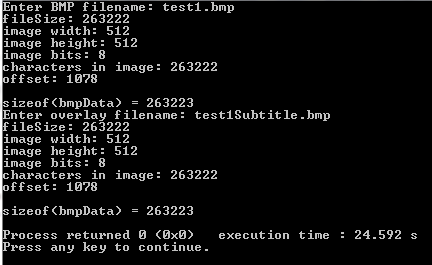
\includegraphics[width=\linewidth]{prompt.png}
  \captionof{figure}{Sample run of "test1.bmp"}
\end{Figure}


\begin{Figure}
 \centering
 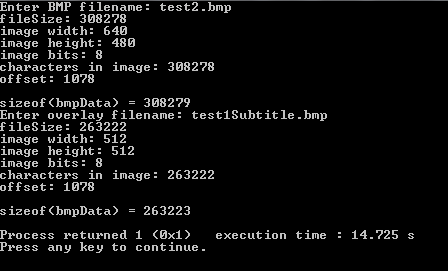
\includegraphics[width=\linewidth]{prompt2.png}
  \captionof{figure}{Sample run of "test2.bmp"}
\end{Figure}

{\bf Structure of a Bitmap  File:}
The BMP files we will be working with here consist of three parts: the header, the information section, and the pixel data. The 54 byte header contains the following information about the BMP file:

\begin{center}
\begin{tabular}{| l | l | l | }
\hline
  Offset & Size & Description\\ \hline
  2 & 4  & Size of BMP (bytes) \\
  10 & 4 & Offset to Start of Pixel Data (bytes)\\
18 & 4 & Image Width (pixels)\\
22 & 4 & Image Height (pixels)\\
28 & 2 & Number of Bits per Pixel \\
\hline
\end{tabular}
\end{center}

The information section is noted but not used in this program. The pixel data begins at the byte obtained from the offset to the start of the pixel data retrieved through the header. The pixel data is an array of pixels (height multiplied by width) where each pixel has the format of the 8 bit (number of bits per pixel) grayscale. The grayscale is a range from 0 to 255, where 0 is black and 255 is white. 

{\bf Reading a Bitmap File:}
First, from main(), the first 8-bit grayscale image file is read into, with the function readBM(), an instance of the Image class named original. The readBM function initializes the metadata obtained from the header for that image. The metadata includes the width of the image (imageWidth), the height of the image (imageHeight), the amount of bits for the image (imageBits), the offset between the header and the pixels of the image (offset), a vector of all of the bytes extracted from the image (bmpData), a integer array of the bytes of the header (header[]), and a two-dimensional vector of all of the pixel bytes (pixels). If either image file does not exist or cannot be read, the program will terminate at this point. The second 8-bit grayscale image file name is saved in the variable filename

{\bf Image Overlay:}
Next, from main(), the overlay() function is called on the original image with the overlay filename as the parameter. Within the overlay() function, an instance of the Image class, foreground, is created for the overlay BMP file. The readBM() function is called on the foreground Image using the filename as the parameter. This initializes all of the data types for the image to overlay (foreground) over the original. The twoImageSameDimension() function is called to return turn if the image width and image height are the same. If these two values are not the same, the function will cease to move on and exit. The overlay() function then iterates through the two-dimensional vector of pixels of the foreground and original Image. Anywhere there is a value of 0 (black) in the foreground Image pixels, the original Image pixel is replaced with 255 (white). The overlaid image is then printed to a new file, out1.bmp, with the original image overlaid by the foreground image, changing the foreground image from black to white.

{\bf Image Histogram Equalization:}
Next, from main(), the histogramEqualization() function is called on the original image. In the histogramEqualization() function, an array, hist[], is created to count the total number of pixels (height multiplied by width) associated with each pixel intensity (0 to 255) of the original Image. The original image histogram will be used for equalization, stretching the current range of pixels to a full range (between 0 and 255).  An array, cumulative[], is created to calculate the cumulative histogram. The cumulative histogram is the running total of pixel intensities from the array hist[]. Histogram equalization is calculated by the following equation:\\
\[ \text{new value }=  \frac{255\times\text{cumulative histogram value}}{\text{total number of pixels}} \] 
The new pixel values are reassigned using the value obtained by multiplying the maximum intensity by the ratio of the cumulative count at that specific intensity over the total number of pixels. Using the cumulative histogram in the equation allows the pixel values to spread over the maximum range. 
The outputBM() function is called and creates a new BMP file, out2.bmp, with the pixels adjusted by histogram equalization. The results of all functions will be displayed in the Evaluation section.



%----------------------------------------------------------------------------------------
%		EVALUATION
%----------------------------------------------------------------------------------------

\begin{center}
{\large III. Evaluation (Megan Rowland / Michael Micros)}\\
\end{center}

The program functions clearly perform as intended, yielding the expected results. For the overlay function, the user is prompted to enter the filename of the original image and then is asked to enter the filename of the image to be overlaid on the original. The results of the overlay() function called on  the test images overlaid with the overlay images are displayed in Fig. 3  and Fig.4.


\begin{Figure}
 \centering
 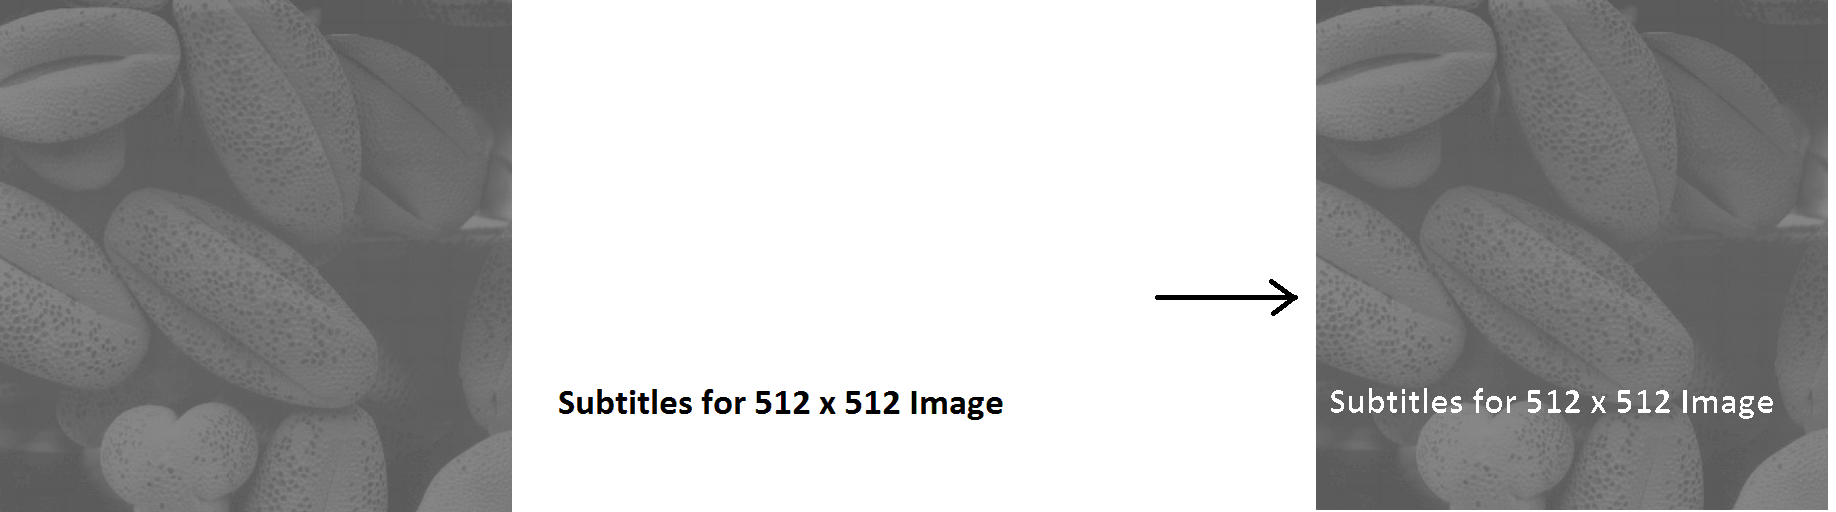
\includegraphics[width=\linewidth]{sample1.png}
  \captionof{figure}{Test1.bmp with overlaid subtitles}
\end{Figure}


\begin{Figure}
 \centering
 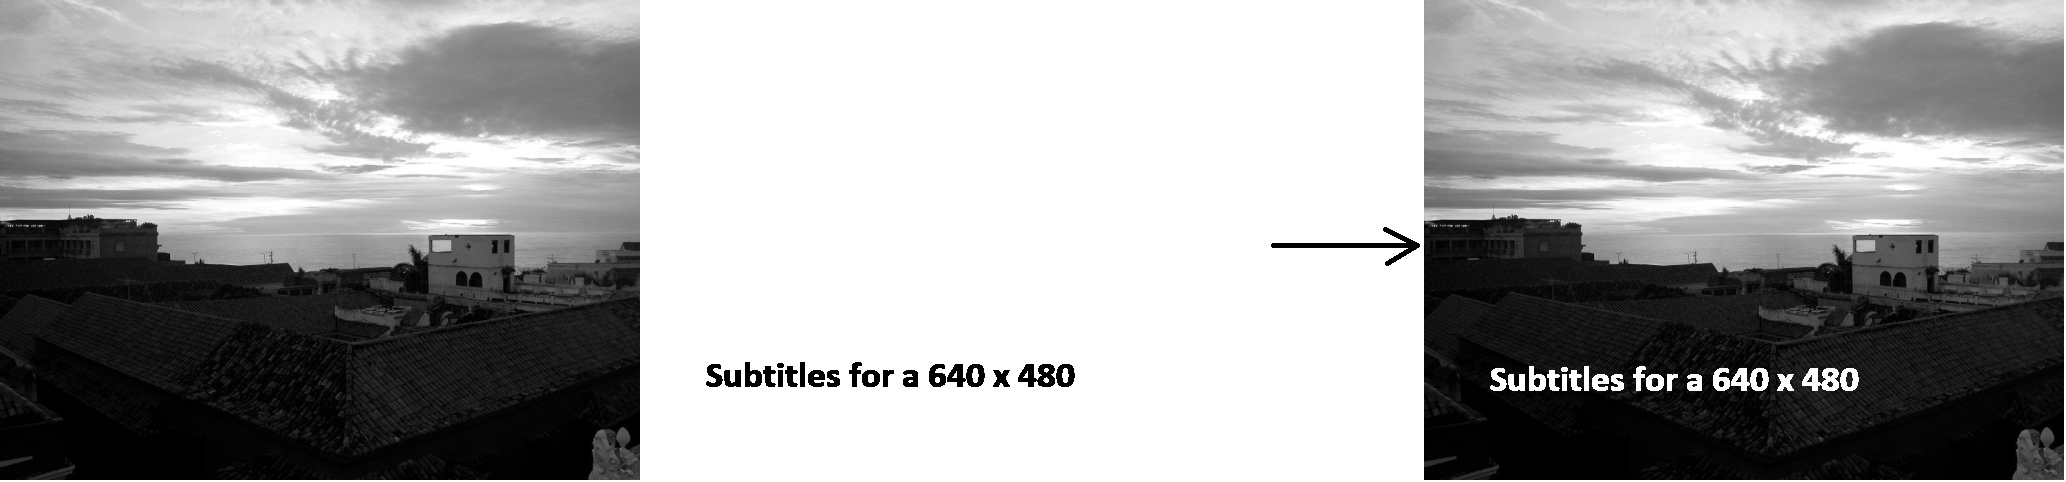
\includegraphics[height=3cm,width=\linewidth]{sample2.png}
  \captionof{figure}{Test2.bmp with overlaid subtitles}
\end{Figure}



As can be seen, the subtitle images are overlaid on top of the originals without altering any of the pixels except those that are needed.
The results from the histogram equalization for both “test1.bmp” and “test2.bmp” are displayed in Fig. 5 and Fig.6. 


\begin{Figure}
 \centering
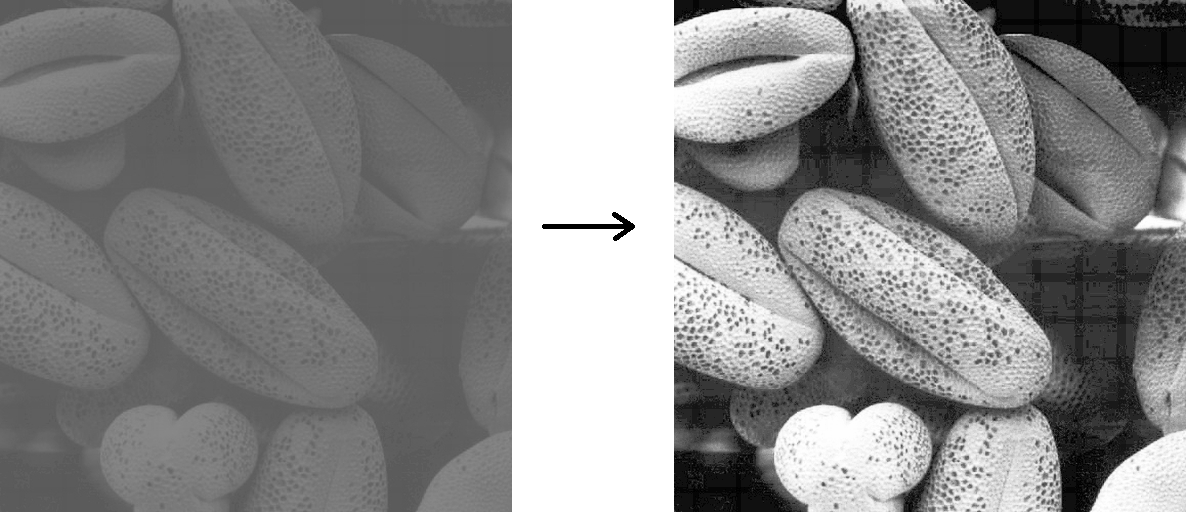
\includegraphics[width=\linewidth]{equal1.png}
  \captionof{figure}{Test1.bmp before and after equalization}
\end{Figure}


\begin{Figure}
 \centering
 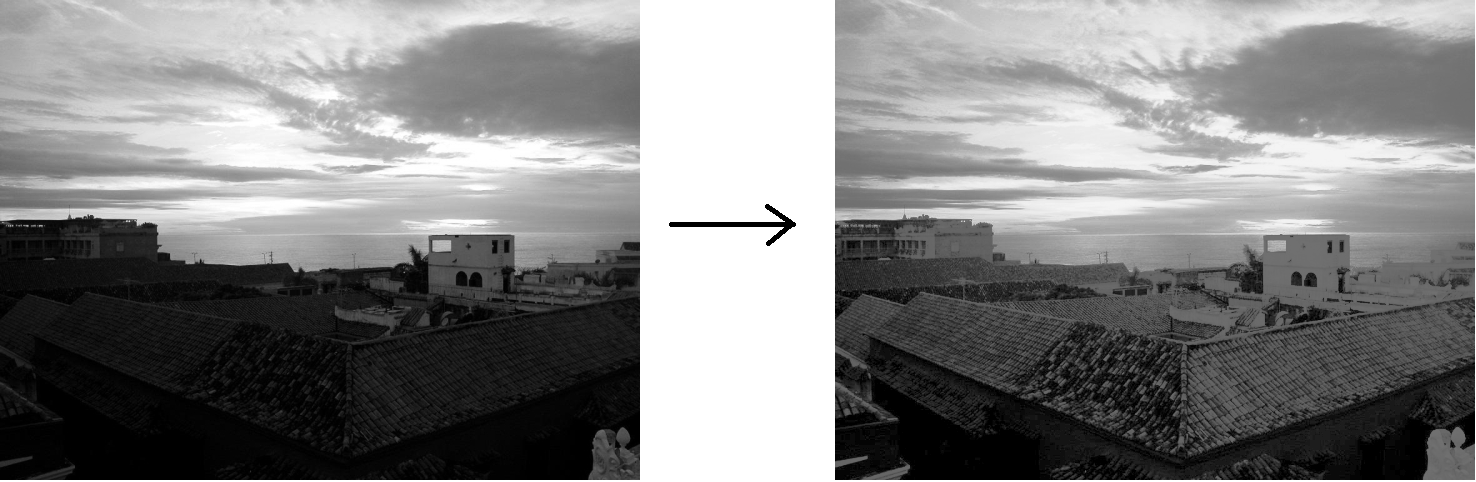
\includegraphics[width=\linewidth]{equal2.png}
  \captionof{figure}{Test2.bmp before and after equalization}
\end{Figure}

The effects of the histogram equalization are noticable when comparing the color distributions before and after the equalization. Notice how at first (Fig. 7) all the colors are distributed only to a limited range of the entire spectrum, specifically in the value range 88 to 139. In histogram equalization the goal is to populate the entire available spectrum of colors (0 to 255) without altering the differences between neiboring colors. This result is seen in Fig. 8. It is important to note that the greater the difference in the number of pixels bewtween neighbouring bins in the original image, the further apart they will be in the equalized histogram. 


\begin{Figure}
 \centering
 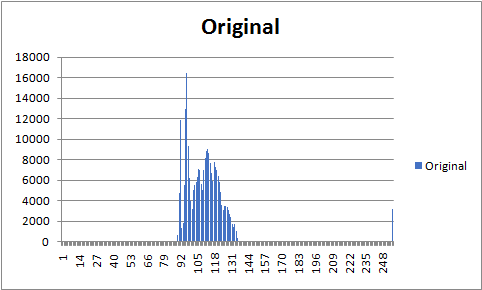
\includegraphics[width=\linewidth]{hist1.png}
  \captionof{figure}{Histogram of original test1.bmp}
\end{Figure}


\begin{Figure}
 \centering
 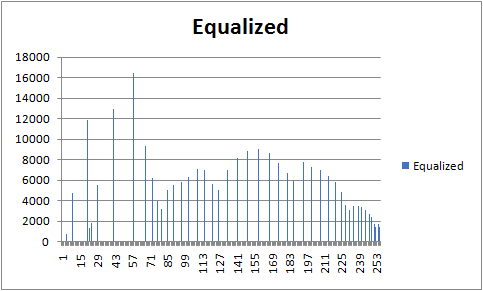
\includegraphics[width=\linewidth]{eqHist.png}
  \captionof{figure}{Histogram of equalized test1.bmp}
\end{Figure}


\vspace{15 pt}

%----------------------------------------------------------------------------------------
%		DISCUSSION
%----------------------------------------------------------------------------------------


\begin{center}
{\large IV. Discussion (Michael Micros)}
\end{center}

Based on the results presented in the Evaluation the overlay function works exactly as intended, without much room for improvement. The only scenario in which a problem may arise is when it is required to overlay an image that is very bright or completely white in the area that the overlaid image will affect. A situation like this could make difficult to make out the subtitles or overlaid image. Such a problem can be easily solved by adding an outline to the overlay image (around the subtitles for our particular implementation) of a different color. For example, if in the overlay image a pixel value of 255 is detected, the pixel from the original image will appear in the output image. If a pixel value of  0 is detected, a white pixel will appear in the output image. Finally, if a pixel value of 128 (an arbitrary value we select for the outline of the text) is detected, a black pixel will appear in the output image. This will provide a black outline to the white overlay that we have chosen.

As for the histogram equalization, even though the resulting images seem to provide a more equal distribution of color it is obvious that better results could be achieved by implementing a more complex equalization technique. By comparing the histograms of the original and equalized image it is important to note that when the number of pixels is very small for colors that are very similar, those pixels may end up having the same color in the equalized image. This does not exactly violate any of the restrictions that were imposed, and sometimes may be desirable. Another observation that can be made is that when performing histogram equalization, in order to improve the contrast in a large area we sacrifice the contrast in a smaller area of the image. An example of this can be seen in the bottom right corner of “test2.bmp” and its equalized counterpart.

%----------------------------------------------------------------------------------------
%		APPENDIX
%----------------------------------------------------------------------------------------


\begin{center}
{\large V. Appendix}
\end{center}

\end{multicols*}

\begin{figure}[h]
 \centering
 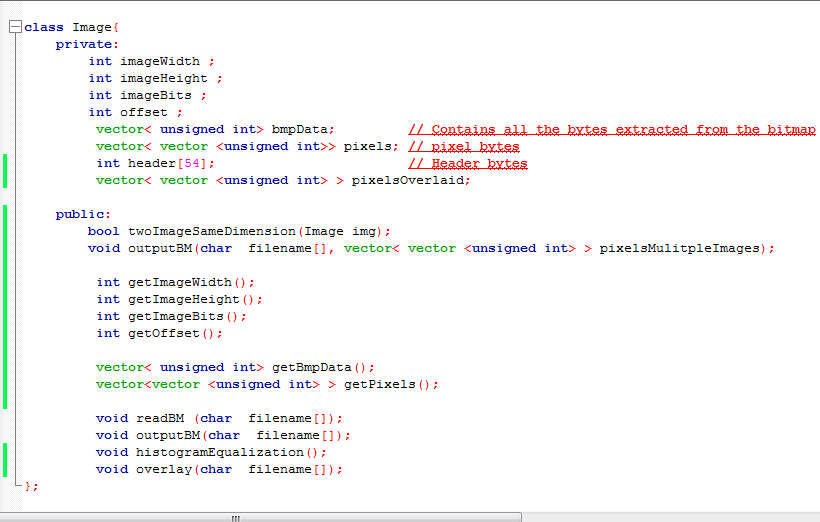
\includegraphics[width=\linewidth]{ImageClass.png}
  \captionof{figure}{Image class}
\end{figure}














%----------------------------------------------------------------------------------------
\end{document}
